\documentclass[conference]{IEEEtran}
\IEEEoverridecommandlockouts
% The preceding line is only needed to identify funding in the first footnote. If that is unneeded, please comment it out.
\usepackage{cite}
\usepackage{amsmath,amssymb,amsfonts}
\usepackage{algorithmic}
\usepackage{graphicx}
\usepackage{textcomp}
\usepackage{xcolor}
\def\BibTeX{{\rm B\kern-.05em{\sc i\kern-.025em b}\kern-.08em
    T\kern-.1667em\lower.7ex\hbox{E}\kern-.125emX}}
\begin{document}

\title{Paper Title*\\
{\footnotesize \textsuperscript{*}Note: Sub-titles are not captured in Xplore and
should not be used}
}

\author{\IEEEauthorblockN{1\textsuperscript{st} Given Name Surname}
\IEEEauthorblockA{\textit{dept. name of organization (of Aff.)} \\
\textit{name of organization (of Aff.)}\\
City, Country \\
email address}
\and
\IEEEauthorblockN{2\textsuperscript{nd} Given Name Surname}
\IEEEauthorblockA{\textit{dept. name of organization (of Aff.)} \\
\textit{name of organization (of Aff.)}\\
City, Country \\
email address}
\and
\IEEEauthorblockN{3\textsuperscript{rd} Given Name Surname}
\IEEEauthorblockA{\textit{dept. name of organization (of Aff.)} \\
\textit{name of organization (of Aff.)}\\
City, Country \\
email address}
}

\maketitle

\begin{abstract}
Write Abstract
\end{abstract}

\begin{IEEEkeywords}
spark,benchmark,resource
\end{IEEEkeywords}

\section{Introduction}
Write Intro

AWS - Charge for resources used.  Execution time and resource usage are related.  Same with CPU Time

%# Note: Use task metrics available through spark so that others can take advantage.
%Write jobs like beginners

\section{Spark Discussion RDD vs Dataset vs DataFrame}
%@Mariama


There are several differences between the three data formats that were used in this project.
Resilient Distributed Dataset (RDD) data is an immutable representation of distributed data.
RDD is best for unstructured data such as text and byte streams.
Datasets in the simplest terms are extensions of the Spark dataframe, and provide an object oriented interface.
DataFrames organize data into columns, and provide a domain-specific API to manipulate distributed data.
Data can be queried from both DataFrames and RDD through Spark SQL.

Regarding the reported performance of the three data formats from other sources,
RDD offer a data format solution that is less expensive than the other data formats.
This is, however, at the sacrifice of data performance. For a more efficient data format, DataFrames and dataset provide
a means of attaining greater optimization.
As specified in later sections, mapping and map partitions are optimizations that can be manually added to RDD
for efficiency.
Datasets in particular provides optimized queries through the Catalyst Query Optimizer (execution agnostic framework).
The above performance notes will be apparent in the visualizations and analysis of the graphs in the pages that follow.

References:
https://databricks.com/blog/2016/07/14/a-tale-of-three-apache-spark-apis-rdds-dataframes-and-datasets.html
https://data-flair.training/blogs/apache-spark-rdd-vs-dataframe-vs-dataset/
https://data-flair.training/blogs/apache-spark-dataset-tutorial/

\subsection{SparkMeasure and Spark 2.4.0}

\section{Data Discussion}
Mention the data and some stats including:
Size in bytes of the input data for local testing (can get this from metrics)
Number of records of the input data for local testing

Mention data preparation + CSV transformation

If we do the cluster, there'll be more data, so we'll want to discuss those stats as well.

Cleanup to fairly enable dataframe


\section{Setup}
%TODO: Get Specs
The local machine is from running on a Mac.

\section{Map vs MapPartitions in RDD}
%TODO: We could describe partitioning in spark in more detail
%TODO: Rewrite sentence below
While writing Spark jobs, it is important to implement code that is efficient.
The Spark jobs written for the purpose of this paper are not necessarily the most efficient, especially since the definition of efficient is somewhat subjective.
This paper explores one definition of efficiency by examining the usage of available resources.
Thus, the question of using the map method versus the mapParititions method is a good starting to place since it will define how the remaining Spark jobs using RDDs get written.

One of the most popular efficiencies is the usage of the mapParititions method instead of the map method when transforming an RDD.
The map method will apply the specified transform to every element in the RDD.
The mapPartitions method operates on a partition of the RDD.
Simply put, a partition is a chunk of data in the RDD that can be operated on all at once without needing to shuffle the data.
So, a mapPartitions method may apply the same transform to every data element within its partition, thus acting like the map method would.
Keep in mind that mapPartitions may be used for more complicated operations utilizing all of the data elements within a partition.

While there are no traditional publications discussing the pros and cons of mapPartitions vs map, the general consensus on popular internet forums is that mapPartitions is generally faster because you do not have to set up a function for every element, just for the partition.

%TODO: Create references
https://stackoverflow.com/questions/21185092/apache-spark-map-vs-mappartitions
https://martin.atlassian.net/wiki/spaces/lestermartin/blog/2016/05/19/67043332/why+spark+s+mapPartitions+transformation+is+faster+than+map+calls+your+function+once+partition+not+once+element
https://www.quora.com/What-is-the-difference-between-a-map-and-mapPartitions-in-Spark

Include graphic explaining what the jobs are

\subsection{Running on Local Machine}

\subsubsection{Execution Time Comparison}
The execution time of the Spark job can be found by subtracting the minimum value of the launchTime stat from the maximum of the finishTime stat.

\begin{figure}
    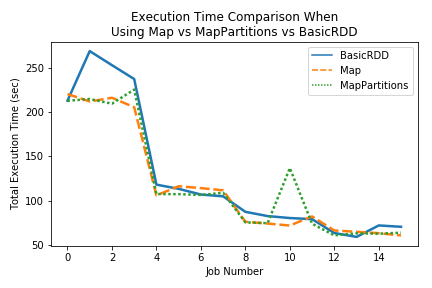
\includegraphics[width=\linewidth]{../python_scripts/images/mapVsMapPartitionsAllExecutionTime.png}
    \caption{Comparison of Map job vs MapPartitions job vs Basic RDD job}
    \label{fig:mapVMapPartitionsAllExecTime}
\end{figure}

The focus of this paper is on the importance of using benchmarks other than execution time for Spark analytics and Figure \ref{fig:mapVMapPartitionsAllExecTime} exemplifies this motivation by showing that:
\begin{itemize}
\item Even the exact same Spark analytic, such as the Basic RDD job and the MapPartitions job, may not consistently have the same execution time.
\item There can be anomalies in the execution time, which is likely due to the interference of other proccesses running on the same machine.
\end{itemize}

Additionally, Figure \ref{fig:mapVMapPartitionsAllExecTime} also shows that there is, as expected, a relationship between the number of threads running the job and the execution time.
For instance, doubling the threads from 1 to 2 cut the execution time in half.
Tripling the threads from 1 to 3 reduced the execution time to about a third of the execution time of 1 thread.
Increasing the number of threads from 1 to 4 also resulted in the run time decreasing to about 25\% of the original run time.

This confirms that increasing the parallelization of the job by increasing the number of threads will decrease the run time;
however, this does not confirm the commonly held belief that the mapPartitions method will execute faster than map method.
This transitions to the next question analyzed of whether there is an advantage when it comes to the peak execution memory.

\subsubsection{Peak Execution Memory Comparison}
\begin{figure}
    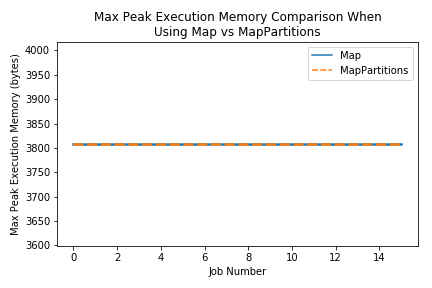
\includegraphics[width=\linewidth]{../python_scripts/images/mapVsMapPartitionsMaxPeakExecutionMemory.png}
    \caption{A boat.}
    \label{fig:mapVMapPartitionsMaxPeakExecutionMemory}
\end{figure}

%TODO: Should probably explain why max peak execution memory is the stat we focus on.
%TODO: Maybe dig deeper into this stat.  Why is it the same for all jobs.
Figure \ref{fig:mapVMapPartitionsMaxPeakExecutionMemory} shows that the peak execution memory is the same for both map and mapPartitions.
Since this is the case, the remaining Spark jobs working with RDDs will utilize mapPartitions instead of map.

%TODO: The comparison of the peakExecutionMemory vs BytesWritten for this job was interesting. Can use as space filler.
%-We may also want to look at some other memory metrics available

%TODO: Decide if we want to do the following CPU Time Comparison
%\subsubsection{CPU Time Comparison}
%\begin{figure}
%    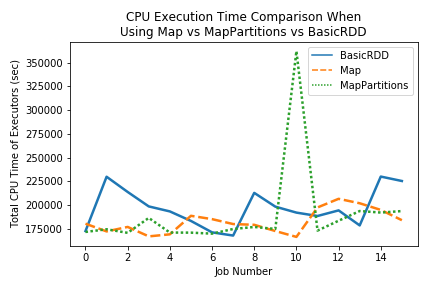
\includegraphics[width=\linewidth]{../python_scripts/images/mapVsMapPartitionsAllCpuTime.png}
%    \caption{A boat.}
%    \label{fig:boat1}
%\end{figure}

%\subsection{Running on Distributed Cluster}
%\subsubsection{Resource Usage Comparison}
%\subsubsection{Execution Time Comparison}
%
%Might be worthwhile to create another job that would call a toList on the partition iterator.

\section{Basic RDD vs Dataset vs Dataframe}\label{basicjobs}
The equivalent of the Hello World program for any big data analytics platform, including Spark, is Word Count.
The basic premise of the Word Count program is to count all of the unique words in a document.
The NOAA GSOD data does not easily support a Word Count program, so instead, a similar program was created to start the analysis of the peak execution memory for RDDs, DataFrames and Datasets.
In this job, a key was created by combining the station number and the nearest multiple of 10 of the average temperature that does not go over the average temperate (Ex 98 $\rightarrow$ 90).
Each unique key is the counted.
The output of the program is a count of all of the unique keys as this will force the program to run in its entirety to ensure equal comparison.

\subsection{Running on Local Machine}

\subsubsection{Peak Execution Memory Comparison}
Create a bar graph or line graph with 3 options to compare RDD vs dataframe vs dataset and the jobs per peakExecutionMemory

\subsubsection{Execution Time Comparison}
Create a bar graph or line graph with 3 options to compare RDD vs dataframe vs dataset and the jobs per execution time

\section{Paritions RDD vs Dataset vs Dataframe}
The partition jobs were basically copies of the "Basic" jobs discussed in Section \ref{basicjobs}; however, the coalesce method was used on the raw input.
The coalesce method was used instead of the repartition method because repartition will force a shuffle.
The coalesce method, in this case, will not force a shuffle and will instead just redistribute the old partitions to the specified number of new partitions.
Coalesce was the chosen method because even in the smaller job running on a local machine, over 12000 partitions were going to be created.
%TODO: Verify the following sentence.
Furthermore, coalesce was called on the raw input because that is guaranteed to be the one part that's shared between all of the jobs in this case;
however, Datasets and DataFrames have their own internal optimizations that may move that coalesce.

\subsection{Compare Specified Partitions with True Partitions}
The jobs look like we may have said "do x partitions", but it only create y partitions. This should be explored.
Can we create a graphic for this?

\subsection{Resource Comparison for different partitions}
Create a line graph with 3 options to compare RDD vs dataframe vs dataset and the jobs per peakExecutionMemory

\subsection{Execution Time Comparison}
Create a line graph with 3 options to compare RDD vs dataframe vs dataset and the jobs per peakExecutionMemory for execution time


\section{Cache RDD vs Dataset vs Dataframe}

Talk about the job. Basically a grouping + count + count.  Discuss where the caching happens.

\subsection{Discuss Issues with Caching}
It looks like data had to spill to disk during the caching. We need to discuss this and other metrics that could be used
to explain this behavior.

\subsection{Resource Comparison for different partitions}
Create a line graph with 3 options to compare RDD vs dataframe vs dataset and the jobs per peakExecutionMemory.  Need to explore other metrics

\subsection{Execution Time Comparison}
Create a line graph with 3 options to compare RDD vs dataframe vs dataset and the jobs per peakExecutionMemory for execution time. Need to explore other metrics

Should we explore other caching levels?
%https://spark.apache.org/docs/2.1.0/api/scala/index.html#org.apache.spark.rdd.RDD@persist(newLevel:org.apache.spark.storage.StorageLevel):RDD.this.type

There's also joins

And we can discuss KMeans since those jobs were run.
























\subsection{Abbreviations and Acronyms}\label{AA}
Define abbreviations and acronyms the first time they are used in the text, 
even after they have been defined in the abstract. Abbreviations such as 
IEEE, SI, MKS, CGS, ac, dc, and rms do not have to be defined. Do not use 
abbreviations in the title or heads unless they are unavoidable.

%\subsection{Units}
%\begin{itemize}
%\item Use either SI (MKS) or CGS as primary units. (SI units are encouraged.) English units may be used as secondary units (in parentheses). An exception would be the use of English units as identifiers in trade, such as ``3.5-inch disk drive''.
%\item Avoid combining SI and CGS units, such as current in amperes and magnetic field in oersteds. This often leads to confusion because equations do not balance dimensionally. If you must use mixed units, clearly state the units for each quantity that you use in an equation.
%\item Do not mix complete spellings and abbreviations of units: ``Wb/m\textsuperscript{2}'' or ``webers per square meter'', not ``webers/m\textsuperscript{2}''. Spell out units when they appear in text: ``. . . a few henries'', not ``. . . a few H''.
%\item Use a zero before decimal points: ``0.25'', not ``.25''. Use ``cm\textsuperscript{3}'', not ``cc''.)
%\end{itemize}

%\begin{equation}
%a+b=\gamma\label{eq}
%\end{equation}

%Be sure that the
%symbols in your equation have been defined before or immediately following
%the equation. Use ``\eqref{eq}'', not ``Eq.~\eqref{eq}'' or ``equation \eqref{eq}'', except at
%the beginning of a sentence: ``Equation \eqref{eq} is . . .''

%\subsection{\LaTeX-Specific Advice}
%
%Please use ``soft'' (e.g., \verb|\eqref{Eq}|) cross references instead
%of ``hard'' references (e.g., \verb|(1)|). That will make it possible
%to combine sections, add equations, or change the order of figures or
%citations without having to go through the file line by line.
%
%Please don't use the \verb|{eqnarray}| equation environment. Use
%\verb|{align}| or \verb|{IEEEeqnarray}| instead. The \verb|{eqnarray}|
%environment leaves unsightly spaces around relation symbols.
%
%Please note that the \verb|{subequations}| environment in {\LaTeX}
%will increment the main equation counter even when there are no
%equation numbers displayed. If you forget that, you might write an
%article in which the equation numbers skip from (17) to (20), causing
%the copy editors to wonder if you've discovered a new method of
%counting.
%
%{\BibTeX} does not work by magic. It doesn't get the bibliographic
%data from thin air but from .bib files. If you use {\BibTeX} to produce a
%bibliography you must send the .bib files.
%
%{\LaTeX} can't read your mind. If you assign the same label to a
%subsubsection and a table, you might find that Table I has been cross
%referenced as Table IV-B3.
%
%{\LaTeX} does not have precognitive abilities. If you put a
%\verb|\label| command before the command that updates the counter it's
%supposed to be using, the label will pick up the last counter to be
%cross referenced instead. In particular, a \verb|\label| command
%should not go before the caption of a figure or a table.
%
%Do not use \verb|\nonumber| inside the \verb|{array}| environment. It
%will not stop equation numbers inside \verb|{array}| (there won't be
%any anyway) and it might stop a wanted equation number in the
%surrounding equation.
%
%\subsection{Some Common Mistakes}\label{SCM}
%\begin{itemize}
%\item The word ``data'' is plural, not singular.
%\item The subscript for the permeability of vacuum $\mu_{0}$, and other common scientific constants, is zero with subscript formatting, not a lowercase letter ``o''.
%\item In American English, commas, semicolons, periods, question and exclamation marks are located within quotation marks only when a complete thought or name is cited, such as a title or full quotation. When quotation marks are used, instead of a bold or italic typeface, to highlight a word or phrase, punctuation should appear outside of the quotation marks. A parenthetical phrase or statement at the end of a sentence is punctuated outside of the closing parenthesis (like this). (A parenthetical sentence is punctuated within the parentheses.)
%\item A graph within a graph is an ``inset'', not an ``insert''. The word alternatively is preferred to the word ``alternately'' (unless you really mean something that alternates).
%\item Do not use the word ``essentially'' to mean ``approximately'' or ``effectively''.
%\item In your paper title, if the words ``that uses'' can accurately replace the word ``using'', capitalize the ``u''; if not, keep using lower-cased.
%\item Be aware of the different meanings of the homophones ``affect'' and ``effect'', ``complement'' and ``compliment'', ``discreet'' and ``discrete'', ``principal'' and ``principle''.
%\item Do not confuse ``imply'' and ``infer''.
%\item The prefix ``non'' is not a word; it should be joined to the word it modifies, usually without a hyphen.
%\item There is no period after the ``et'' in the Latin abbreviation ``et al.''.
%\item The abbreviation ``i.e.'' means ``that is'', and the abbreviation ``e.g.'' means ``for example''.
%\end{itemize}
%An excellent style manual for science writers is \cite{b7}.
%
%\subsection{Authors and Affiliations}
%\textbf{The class file is designed for, but not limited to, six authors.} A
%minimum of one author is required for all conference articles. Author names
%should be listed starting from left to right and then moving down to the
%next line. This is the author sequence that will be used in future citations
%and by indexing services. Names should not be listed in columns nor group by
%affiliation. Please keep your affiliations as succinct as possible (for
%example, do not differentiate among departments of the same organization).
%
%\subsection{Identify the Headings}
%Headings, or heads, are organizational devices that guide the reader through
%your paper. There are two types: component heads and text heads.
%
%Component heads identify the different components of your paper and are not
%topically subordinate to each other. Examples include Acknowledgments and
%References and, for these, the correct style to use is ``Heading 5''. Use
%``figure caption'' for your Figure captions, and ``table head'' for your
%table title. Run-in heads, such as ``Abstract'', will require you to apply a
%style (in this case, italic) in addition to the style provided by the drop
%down menu to differentiate the head from the text.
%
%Text heads organize the topics on a relational, hierarchical basis. For
%example, the paper title is the primary text head because all subsequent
%material relates and elaborates on this one topic. If there are two or more
%sub-topics, the next level head (uppercase Roman numerals) should be used
%and, conversely, if there are not at least two sub-topics, then no subheads
%should be introduced.
%
%\subsection{Figures and Tables}
%\paragraph{Positioning Figures and Tables} Place figures and tables at the top and
%bottom of columns. Avoid placing them in the middle of columns. Large
%figures and tables may span across both columns. Figure captions should be
%below the figures; table heads should appear above the tables. Insert
%figures and tables after they are cited in the text. Use the abbreviation
%``Fig.~\ref{fig}'', even at the beginning of a sentence.
%
%\begin{table}[htbp]
%\caption{Table Type Styles}
%\begin{center}
%\begin{tabular}{|c|c|c|c|}
%\hline
%\textbf{Table}&\multicolumn{3}{|c|}{\textbf{Table Column Head}} \\
%\cline{2-4}
%\textbf{Head} & \textbf{\textit{Table column subhead}}& \textbf{\textit{Subhead}}& \textbf{\textit{Subhead}} \\
%\hline
%copy& More table copy$^{\mathrm{a}}$& &  \\
%\hline
%\multicolumn{4}{l}{$^{\mathrm{a}}$Sample of a Table footnote.}
%\end{tabular}
%\label{tab1}
%\end{center}
%\end{table}

%Figure Labels: Use 8 point Times New Roman for Figure labels. Use words
%rather than symbols or abbreviations when writing Figure axis labels to
%avoid confusing the reader. As an example, write the quantity
%``Magnetization'', or ``Magnetization, M'', not just ``M''. If including
%units in the label, present them within parentheses. Do not label axes only
%with units. In the example, write ``Magnetization (A/m)'' or ``Magnetization
%\{A[m(1)]\}'', not just ``A/m''. Do not label axes with a ratio of
%quantities and units. For example, write ``Temperature (K)'', not
%``Temperature/K''.

%\section*{Acknowledgment}
%
%The preferred spelling of the word ``acknowledgment'' in America is without
%an ``e'' after the ``g''. Avoid the stilted expression ``one of us (R. B.
%G.) thanks $\ldots$''. Instead, try ``R. B. G. thanks$\ldots$''. Put sponsor
%acknowledgments in the unnumbered footnote on the first page.

\section*{References}

Please number citations consecutively within brackets \cite{b1}. The 
sentence punctuation follows the bracket \cite{b2}. Refer simply to the reference 
number, as in \cite{b3}---do not use ``Ref. \cite{b3}'' or ``reference \cite{b3}'' except at 
the beginning of a sentence: ``Reference \cite{b3} was the first $\ldots$''

Number footnotes separately in superscripts. Place the actual footnote at 
the bottom of the column in which it was cited. Do not put footnotes in the 
abstract or reference list. Use letters for table footnotes.

Unless there are six authors or more give all authors' names; do not use 
``et al.''. Papers that have not been published, even if they have been 
submitted for publication, should be cited as ``unpublished'' \cite{b4}. Papers 
that have been accepted for publication should be cited as ``in press'' \cite{b5}. 
Capitalize only the first word in a paper title, except for proper nouns and 
element symbols.

For papers published in translation journals, please give the English 
citation first, followed by the original foreign-language citation \cite{b6}.

\begin{thebibliography}{00}
\bibitem{b1} G. Eason, B. Noble, and I. N. Sneddon, ``On certain integrals of Lipschitz-Hankel type involving products of Bessel functions,'' Phil. Trans. Roy. Soc. London, vol. A247, pp. 529--551, April 1955.
\bibitem{b2} J. Clerk Maxwell, A Treatise on Electricity and Magnetism, 3rd ed., vol. 2. Oxford: Clarendon, 1892, pp.68--73.
\bibitem{b3} I. S. Jacobs and C. P. Bean, ``Fine particles, thin films and exchange anisotropy,'' in Magnetism, vol. III, G. T. Rado and H. Suhl, Eds. New York: Academic, 1963, pp. 271--350.
\bibitem{b4} K. Elissa, ``Title of paper if known,'' unpublished.
\bibitem{b5} R. Nicole, ``Title of paper with only first word capitalized,'' J. Name Stand. Abbrev., in press.
\bibitem{b6} Y. Yorozu, M. Hirano, K. Oka, and Y. Tagawa, ``Electron spectroscopy studies on magneto-optical media and plastic substrate interface,'' IEEE Transl. J. Magn. Japan, vol. 2, pp. 740--741, August 1987 [Digests 9th Annual Conf. Magnetics Japan, p. 301, 1982].
\bibitem{b7} M. Young, The Technical Writer's Handbook. Mill Valley, CA: University Science, 1989.
\end{thebibliography}
\vspace{12pt}
\color{red}
IEEE conference templates contain guidance text for composing and formatting conference papers. Please ensure that all template text is removed from your conference paper prior to submission to the conference. Failure to remove the template text from your paper may result in your paper not being published.

\end{document}
